% -----------------------------------------------------------------------
% --- DOCUMENTS ---
% -----------------------------------------------------------------------
\documentclass[francais,12pt]{article}
\usepackage[utf8]{inputenc}
\usepackage{ae, pslatex}
\usepackage[french]{babel}
\selectlanguage{french} 

\usepackage{mathtools}
\usepackage{amssymb}
\usepackage{pgfplots}
\usepackage{caption}
\usepackage{hyperref}
\hypersetup{
    colorlinks=true,
    linkcolor=blue,
    filecolor=magenta,      
    urlcolor=cyan,
}

\usepackage{titlesec}
\usepackage{color}
\usepackage{colortbl}

\usepackage{hhline,tabu}

% -----------------------------------------------------------------------
% --- CODE JAVA ---
% -----------------------------------------------------------------------
\usepackage{listings} % pour afficher du code
\definecolor{mauve}{rgb}{0.472,0.035,0.218}
\definecolor{darkGreen}{rgb}{0.0429,0.601,0.0117}
\definecolor{antiFlashWite}{rgb}{0.95,0.95,0.96}
 

\lstdefinelanguage{Java}{
	morekeywords={typeof, new, true, false, catch, function, return, null, catch, switch, var, if, in, while, do, else, case, break, let,this},
	morecomment=[s]{/*}{*/},
	morecomment=[l]//,
	morestring=[b]",
	morestring=[b]',
	morestring=[s]{/[}{/;}
}

\lstdefinestyle{javaCode}
{
	% language related
	language=Java,
	keywordstyle=\color{blue},
	commentstyle=\color{green},
	stringstyle=\color{mauve},
	basicstyle=\footnotesize\ttfamily, % Standardschrift
	numbers=left,               % Ort der Zeilennummern
	numberstyle=\tiny,          % Stil der Zeilennummern
	stepnumber=2,               % Abstand zwischen den Zeilennummern
	numbersep=5pt,              % Abstand der Nummern zum Text
	tabsize=4,                  % Groesse von Tabs
	extendedchars=true,         %
	breaklines=true,            % Zeilen werden Umgebrochen
	keywordstyle=\color{blue}\bfseries,
	frame=b,
	showspaces=false,           % Leerzeichen anzeigen ?
	showtabs=false,             % Tabs anzeigen ?
	xleftmargin=17pt,
	framexleftmargin=17pt,
	framexrightmargin=5pt,
	framexbottommargin=4pt,
	backgroundcolor=\color{antiFlashWite},
	showstringspaces=false,      % Leerzeichen in Strings anzeigen ?
}

% -----------------------------------------------------------------------
% --- MARGES ---sp
% -----------------------------------------------------------------------
\usepackage{vmargin}
\setpapersize{A4}
\setmarginsrb{60pt}{50pt}{60pt}{25pt}{15pt}{25pt}{15pt}{25pt}

% -----------------------------------------------------------------------
% --- EN-TETE ET PIED DE PAGE ---
% -----------------------------------------------------------------------
\usepackage{fancyhdr}
\usepackage{lastpage}
\pagestyle{fancy}

\fancyhead[L]{SYM - Systèmes mobiles}
\fancyhead[R]{IL - TIC - HEIG-VD \\ Automne 2017}
\fancyfoot[C]{\thepage{}}

\title{Systèmes mobiles \\ Laboratoire n\textordmasculine1 : Introduction aux activités Android}
\author{Mathieu Monteverde, Sathiya Kirushnapillai, Michela Zucca}
\date{Automne 2017}

\titlespacing\section{0pt}{12pt plus 4pt minus 2pt}{0pt plus 2pt minus 2pt}
\titlespacing\subsection{0pt}{12pt plus 4pt minus 2pt}{0pt plus 2pt minus 2pt}
\titlespacing\subsubsection{0pt}{12pt plus 4pt minus 2pt}{0pt plus 2pt minus 2pt}


% ***********************************************************************
% *** DOCUMENT PRINCIPAL ***
% ***********************************************************************
\begin{document}

	\maketitle
    
    \setlength{\parskip}{1em}
    
    \section*{Questions 1}

        Comment organiser les textes pour obtenir une application multi-langues (français, allemand, italien, langue par défaut : anglais)? Que se passe-t-il si une traduction est manquante? \par
        
        {\color[rgb]{0,0.5,0.23}\textbf{Réponse}}
        
        Android permet de gérer les textes et leurs traductions associées à l'aide de fichier \textit{strings.xml}. Pour chaque traduction, il suffit de créer un fichier \textit{strings.xml} et de le placer dans le dossier values-*. Par exemple, values-es pour l'espagnol.\par

        Cette structure correspond à la syntaxe créée par Android Studio en utilisant l'outil de traduction de langue. La langue par défaut se trouve dans le dossier values. C'est cette dernière qui est utilisée si la traduction est manquante.
        
        \textbf{Source}
        
        
        \href{https://developer.android.com/studio/write/translations-editor.html}{Translations Editor - Android Studio officiel}
        

	\section*{Question 2}
		Dans l'exemple fourni, sur le dialogue pop-up, nous affichons l'icône $android.R.drawable.ic\_dialog\_alert$, disponible dans le SDK Android mais qui n'est pas très bien adaptée visuellement à notre utilisation. Nous souhaitons la remplacer avec notre propre icône, veuillez indiquer comment procéder. Dans quel(s) dossier(s) devons-nous ajouter cette image? Décrivez brièvement la logique derrière la gestion des ressources de type "image" sur Android. 
		
		{\color[rgb]{0,0.5,0.23}\textbf{Réponse}}
		
		Note : Nous avons utilisé un fichier .svg pour répondre à cette question.
		
		Pour ajouter le pictogramme au projet, il faut faire un clic droit sur le dossier res, puis cliquer sur $New > Vector Asset > Local file >$ Sélectionner le fichier sur l'ordinateur. 
		
		Cela ajoute l'icône dans le dossier $res/drawable. $
		
		Android utilise des ressources $Drawable$. Une ressource $Drawable$ est un concept général pour un élément graphique qui peut être dessiné sur l'écran. Les images font partie de cette catégorie. 
		
		Android permet également de gérer des set d'icônes adaptés aux différentes densités d'écrans existantes sur le marché. On peut ainsi spécifier les images à utiliser pour les écrans à low-density, medium-density, high-density et Extra-high-density. 
		
		\textbf{Source}

        \href{https://developer.android.com/guide/topics/resources/drawable-resource.html}{Drawable Resources - Android Studio officiel}
		
	\section*{Question 3}
		Lorsque le login est réussi, vous êtes censé chaîner une autre Activity en utilisant un Intent. Si je presse le bouton "Back" de l'interface Android, que puis-je constater ? Comment faire pour que l'application se comporte de manière plus logique ?
		
		{\color[rgb]{0,0.5,0.23}\textbf{Réponse}}
        
		Avec le code fourni, le fait d'appuyer sur le bouton "Back" de l'interface Android a pour effet de revenir à l'écran d'accueil d'Android. 
		
		On aimerait en effet plutôt revenir à l'écran de login par exemple. Pour ce faire il suffit d'enlever l'instruction 
		
		\begin{lstlisting}[style=javaCode]
		finish();
		\end{lstlisting}
		
		qui a pour effet de terminer l'activité principale après l'appel à l'activité de succès. En enlevant cette ligne, l'activité principale reste sur la pile d'activités, et le bouton "Back" permet ainsi d'y revenir depuis l'activité de succès.
		
		
	\section*{Question 4}
		 On pourrait imaginer une situation où cette seconde Activity fournit un résultat (par exemple l'IMEI ou une autre chaîne de caractères) que nous voudrions récupérer dans l'Activity de départ. Comment procéder ? 
		 
		 {\color[rgb]{0,0.5,0.23}\textbf{Réponse}}
		 
		 Pour ce faire il faut dans un premier temps appeler l'activité secondaire avec la méthode 
		 
		 \begin{lstlisting}[style=javaCode]
		 startActivityForResult(...);
		 \end{lstlisting}
		 
		 plutôt que 
		 		 
		 \begin{lstlisting}[style=javaCode]
		 startActivity(...);
		 \end{lstlisting}
		 
		 Cela permet, dans l'activité secondaire, de définir un résultat qui pourra être récupéré depuis l'activité de départ. Pour se faire il suffit de spécialiser la méthode 
		 
		\begin{lstlisting}[style=javaCode]
		 onActivityResult(...);
		 \end{lstlisting}
		 
		 pour récupérer le contenu de ce résultat (voir le code source correspondant dans MainActivity). On notera qu'il est important de vérifier le code de retour passé en paramètre de cette méthode avant de chercher à récupérer les données. Cela permet de savoir si l'activité s'est terminée en nous fournissant un résultat ou non.\newline
		 
		 Pour effectuer cette manipulation, nous avons ajouté un bouton dans la SuccessActivity, dont le seul but est de terminer l'activité en retournant une String.
		 
		\textbf{Source}

        \href{https://stackoverflow.com/questions/13178056/get-data-from-another-activity}{Get data from another activity - Stackoverflow}
    
        \href{https://stackoverflow.com/questions/920306/sending-data-back-to-the-main-activity-in-android}{Sending data back to the Main Activity in android - Stackoverflow}
        
	\section*{Question 5}
		Vous noterez que la méthode $getDeviceId()$ du TelephonyManager, permettant d'obtenir l'IMEI du téléphone, est dépréciée depuis la version 26 de l'API. Veuillez discuter de ce que cela implique lors du développement et de présenter une façon d'en tenir compte avec un exemple de code. 
		
		{\color[rgb]{0,0.5,0.23}\textbf{Réponse}}
        
		Une méthode dépréciée est une méthode considérée obsolète. Elle est conservée dans les versions plus récentes du langage pour deux raisons. La première, laisser le temps nécessaire aux développeurs pour modifier leur code. La seconde pour des raisons de rétro-compatibilité. Elle peut disparaitre à tout moment, il est déconseillé d'utiliser ces méthodes. 
		
		L'impact sur le code en utilisant des méthodes dépréciées, est le risque qu'à tout moment celui-ci ne fonctionne plus correctement. Il est préférable d'utiliser les nouvelles méthodes de remplacement.\newline		
		 \begin{lstlisting}[style=javaCode]
		// MainActivity.java file
		TelephonyManager telManager = (TelephonyManager)getSystemService(Context.TELEPHONY_SERVICE);
		String imei="";
		
		if (android.os.Build.VERSION.SDK_INT >= 26)
			imei = telManager.getImei();
		else
			imei = telManager.getDeviceId();
				
		// AndroidManifest.xml file
		<uses-permission android:name="android.permission.READ_PHONE_STATE"></uses-permission>
		\end{lstlisting}
	
		\textbf{Source}
	
		\href{https://fr.wikipedia.org/wiki/Dépréciation_(informatique)}{Wikipédia - Dépréciation (informatique)}	

		
	\section*{Question 6}
		Dans l'activité de login, en plaçant le téléphone (ou l'émulateur) en mode paysage (landscape), nous constatons que les 2 champs de saisie ainsi que le bouton s'étendent sur toute la largeur de l'écran. Veuillez réaliser un layout spécifique au mode paysage qui permet un affichage mieux adapté et indiquer comment faire pour qu'il soit utilisé à l'exécution.  
		
		{\color[rgb]{0,0.5,0.23}\textbf{Réponse}}
        
        Afin d'avoir un layout spécifique en mode paysage, il suffit de créer un layout (fichier xml) ayant le même nom dans un dossier layout-land. Ainsi, Android utilisera les fichiers spécifiques à l'exécution.
        
        Pour ce laboratoire, nous avons un fichier authent.xml dans un dossier layout-land dans le dossier res.
		
		\textbf{Source}
        
        \href{https://developer.android.com/training/basics/supporting-devices/screens.html}{Supporting Different Screens - Android Studio Officiel}
		
	\section*{Question 7}
		Le layout de l'interface utilisateur de l'activité de login qui vous a été fourni a été réalisé avec un LinearLayout à la racine. Nous vous demandons de réaliser un layout équivalent utilisant cette fois-ci un RelativeLayout.  
		
		{\color[rgb]{0,0.5,0.23}\textbf{Réponse}}
        
		Pour répondre à cette question, l'interface de login fournie en format portrait a été remplacée par
une structure utilisant un RelativeLayout. Grâce à ce layout, il suffit de définir pour chaque élément où il se situe par rapport à son parent ou à ses pairs. Le champ de mot de passe se situe donc par exemple en dessous du champ d'utilisateur. 
		
		\textbf{Source}
        
        \href{https://developer.android.com/guide/topics/ui/layout/relative.html}{Relative Layout - Android Studio Officiel}
		
		\newpage
	\section*{Question 8}
		Implémenter dans votre code les méthodes onCreate(), onStart(), onResume(), onPause(), onStop(), etc... qui marquent le cycle de vie d'une application Android, et tracez leur exécution. Décrivez brièvement à quelles occasions ces méthodes sont invoquées. Si vous aviez (par exemple) une connexion Bluetooth (ou des connexions bases de données, ou des capteurs activés) ouverte dans votre Activity, que faudrait-il peut-être faire, à votre avis (nous ne vous demandons pas de code ici) ? 
		
		{\color[rgb]{0,0.5,0.23}\textbf{Réponse}}
        
		Il y a 3 grandes périodes dans le cycle de vie d'une application. La période dite active, qui peut être interrompue par la période suspendue qui elle-même peut être interrompue par la période arrêtée.
		L'entrée dans chaque état est symbolisée par une méthode et la sortie de chaque état est symbolisée par une autre méthode. Ce que l'on initialise dans le premier état doit presque toujours être stoppé dans le suivant.
		
		\begin{itemize}
			\item La période active : l'activité est simplement sur le dessus de la pile, c'est ce que l'utilisateur consulte et utilise. 
			\item la période suspendue : débute avec $onResume$ et se termine avec $onPause$. Dès que l'activité n'est plus complètement visible, par exemple l'apparition d'une boite de dialogue. Cette période est fréquente il faut donc qu'elle soit rapide et qu'elle utilise peu le processeur.
			\item la période arrêté : l'activité n'est plus visible, mais elle n'est pas à proprement parlé arrêtée. Par exemple un changement d'application. Elle débute par la méthode $onStop$ toujours précédé des méthodes $onResume$ et $onPause$. Elle se poursuit soit par $onRestart$ (retour de l'application en premier plan) ou par la méthode $onDestroy$ (pour libérer des ressources nécessaires) et devra repasser par la méthode $onCreate$ lors du retour au premier plan.
		\end{itemize}
		
			\textbf{Description des méthodes :}
		\begin{itemize}
			\item onCreate : la première à être appelée. Cette méthode est utilisée au démarrage de l'activité pour initialiser les interfaces, récupérer les données (en base de données) et pour démarrer les activités d'arrière-plan qui s'exécutent durant la durée de vie.
			\item onRestart : cette méthode est appelée par une application en arrière-plan. Elle permet de récupérer l'état de l'application et de le recharger lorsque l'application repasse au premier plan.
			\item onStart: cette méthode permet de démarrer l'application préalablement chargée par $onCreate$ ou par $onRestart$.
			\item onResume : cette méthode est appelée à chaque fois que l'activité passe au premier plan, ou à chaque lancement. Elle est utilisée pour initialiser les ressources qui seront coupées par la méthode $onPause$. 
			\item onPause : cette méthode est appelée dès qu'une autre activité se place au premier plan, elle permet de libérer des ressources (mémoire, outils, processeur). Cette méthode peut-être fréquemment appelée il est donc déconseillé de faire des sauvegardes en base de données, car celles-ci sont trop gourmandes en temps.
			\item onStop : cette méthode est appelée lorsque l'application n'est plus du tout visible. C'est ici qu'il faut faire les sauvegardes en bases de données. L'état suivant pouvant être $onDestroy$ en cas de besoin de ressources. 
			\item onDestroy : cette méthode représente la fin de vie de l'activité. Elle peut être appelé délibérément (finish) ou involontairement par le système pour libérer de la mémoire nécessaire au bon fonctionnement de l'appareil.\newline
		\end{itemize}
	
		\begin{center}
			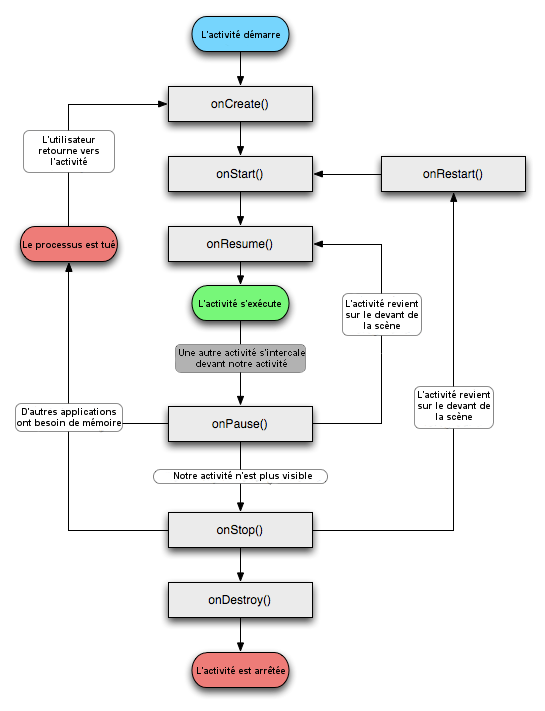
\includegraphics[width=0.9\linewidth]{images/cycleVie}
		\end{center}	
		
		\textbf{Source}
        
        \href{https://openclassrooms.com/courses/creez-des-applications-pour-android/preambule-quelques-concepts-avances}{Application Android - Openclassrooms}
        
\end{document}

